\subsection{前端控制器模式}

前端控制器模式是一种设计模式,它用于处理应用程序中的用户请求。它是一种中央控制器,它能够处理所有请求并将它们分发给相应的处理器。

前端控制器模式的应用场景主要是在Web应用程序中,它能够将用户的请求转发到相应的控制器处理,并返回处理结果给用户。

前端控制器模式的优点是能够提高应用程序的灵活性和可扩展性,并且能够有效地解决请求分发问题。缺点是实现起来比较复杂,需要维护多个控制器和处理器,并且需要花费更多的时间和精力进行设计和实现。

总的来说,前端控制器模式是一种非常有用的设计模式,它能够有效地处理用户请求并将其分发到相应的处理器,提高应用程序的灵活性和可扩展性。

\begin{figure}[H]
  \centering
  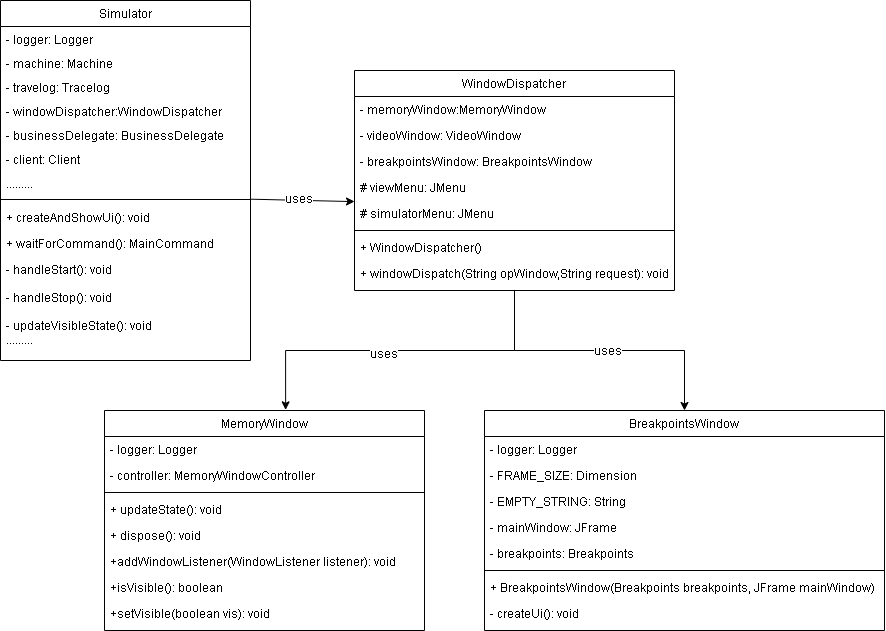
\includegraphics[width=0.9\textwidth]{figures/前端控制器模式.png}
  \caption{前端控制器模式在 Slow6502 中的类图}
\end{figure}